\documentclass[12pt,a4paper,notitlepage]{article}
\usepackage[utf8]{inputenc}
\usepackage{amsmath}
\usepackage{amsfonts}
\usepackage{longtable}
\usepackage{amssymb}
\usepackage{graphicx}
\usepackage[a4paper, left=.6in,right=.6in,top=.8in,bottom=.8in,]{geometry}
\usepackage{tabularx,ragged2e,booktabs,caption}
\usepackage{setspace}
\setstretch{1.5}
\usepackage{tabularx, booktabs}
\usepackage{dcolumn} 
  \newcolumntype{d}[1]{D{.}{.}{#1}}    
\newcolumntype{Y}{>{\centering\arraybackslash}X}
\usepackage[T1]{fontenc}
\usepackage{epigraph}
\usepackage{url}
\usepackage[round,sort]{natbib}
\newcommand{\source}[1]{\caption*{\footnotesize Source: {#1}} }
\usepackage{float}
\usepackage[section]{placeins}
\usepackage{ctable}
\newcolumntype{?}{!{\vrule width 2pt}}
  \newcolumntype{d}[1]{D{.}{.}{#1}}  

\begin{document}
\title{How to wage a trade war? \\
Lessons from the Second Hundred Years War}
\author{
  Guillaume Daudin \\ Université Paris-Dauphine \\guillaume.daudin@dauphine.psl.eu		
  \and
  Elisa Tirindelli\footnote{This paper is not part of my PhD dissertation. It is the continuation of my master's thesis which I am now trying to publish with my previous supervisor, as my co-author. My present supervisor in Trinity College is not involved in this project.} \\ Trinity College Dublin  \\ tirindee@tcd.ie
}
\maketitle

\section*{Abstract}

\epigraph{Savez-vous Messieurs ce qu’est une bataille navale ? On se rencontre, on se salue, on se canonne et la mer n’en reste pas moins salée.}{Maurepas, Navy Minister of Louis  \textsc{xv}, 1718-1748}


What made mercantilist warfare effective in its own terms, i.e. by crippling trade of defeated powers?
Our paper explores the Anglo-French experience during the eighteenth century and contributes to disentangle the effects of all the strategies implemented to curtail enemy's trade. Thanks to a new database of French trade statistics\footnote{http://toflit18.hypotheses.org} we have explored the impact on trade of different elements such as naval supremacy, colony loss and regulations over neutral trade, for different countries; the latter proved to be an unexpectedly powerful tool in this context. By exploiting also bilateral trade flows by product available in the dataset we are confident that we will be able to dig deeper in this result.   \\

\cite{jefferson_letter_1823} famously noticed that European nations \textit{were nations of eternal war}.
Indeed, from 1700 to 1825, two years out of three experienced conflict between major European powers \citep{roser_war_2016}.
Rivalry between Great-Britain and France was central, so much as the period between 1688 to 1815 was called the `` Second Hundred Years War ''.
Mercantile rivalry was an important motivation of French wars (\cite{wallerstein_modern_1980, crouzet_guerre_2008}).
Each nation was jealous of the other's commercial success.
The British believed war was a good way to curtail French trade.
The French believed it could be a good way to curtail British trade, but were more wary of wars because they did not have much naval success.
It is not obvious any of the long list of wars between France and Britain after the death of Louis XIV - War of the Polish Succession (1733-1738) (little naval hostilities), War of the Austrian Succession (1740-1748, where naval hostilities started in 1744), Seven Years' War (1756–1763) and the War of American independence (1775–1783, where French involvement started in 1778) achieved their mercantile goal effectively.
Figure \ref{FrBritTrade} shows that French trade, despite a decrease in wartime, was recovering quite fast after each of these four wars.
French Revolutionary Wars (1792–1802) and Napoleonic Wars (1803–1815) were much more decisive in that respect.

\begin{figure}
\caption{French, British trade and Anglo-French wars}
\centering
\includegraphics[scale=.3]{"Total silver trade FR GB".png}
\source{French trade up to 1821: \cite{daudin_toflit18_????}. French trade 1822-1840: \cite{federico_world_2016} / \cite{dedinger_exploring_2017},

England/British trade up to 1800: \cite{deane_british_1969}. UK trade from 1801 to 1840: \cite{federico_world_2016} / \cite{dedinger_exploring_2017},

Livre tournois silver value: \cite{de_wailly_memoire_1857} and \cite{hoffman_priceless_2000}; Pound sterling silver value: \cite{clark_england_1209-1914_2006} and \cite{jastram_silver_1981}}
\label{FrBritTrade}
\end{figure}
 \\
Computing a loss function, however, reveals a slightly different picture.
Loss is defined as the percentage loss compared to past peace time trend:
\begin{equation*}
Loss = \frac{Expected \> value \> based \> on \>past \> peace \>trend - Observed \> value}{Expected \> value \> based \> on \>past \> peace \>trend}
\end{equation*}
 Figure \ref{annual_loss_function} shows the annual loss function for the period of interest. Figure \ref{mean_loss_function} shows the mean loss function by peace or war period.
\begin{center}
\begin{figure}[H]
\caption{Annual Loss Function}
\label{annual_loss_function}
\centering
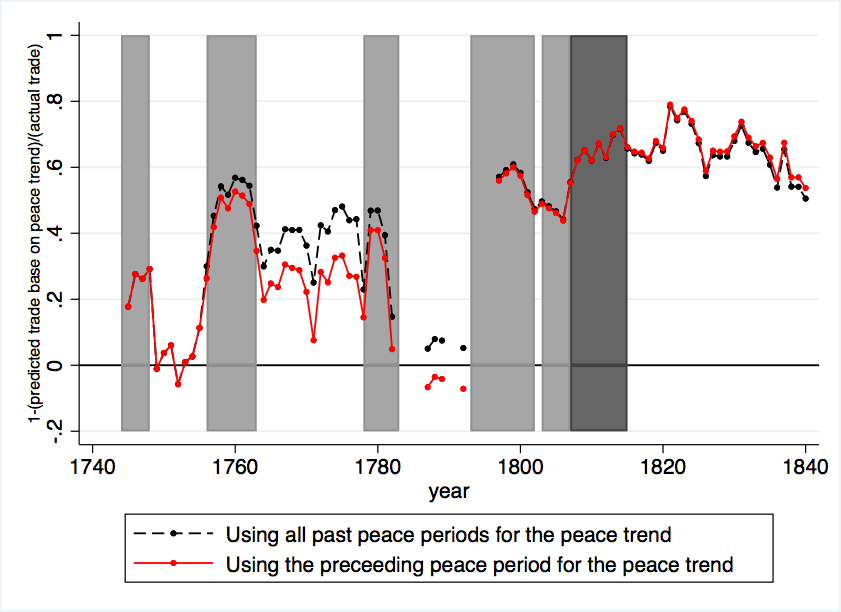
\includegraphics[scale=.3]{Annual_loss_function.png}
\caption{Mean Loss Function}
\label{mean_loss_function}
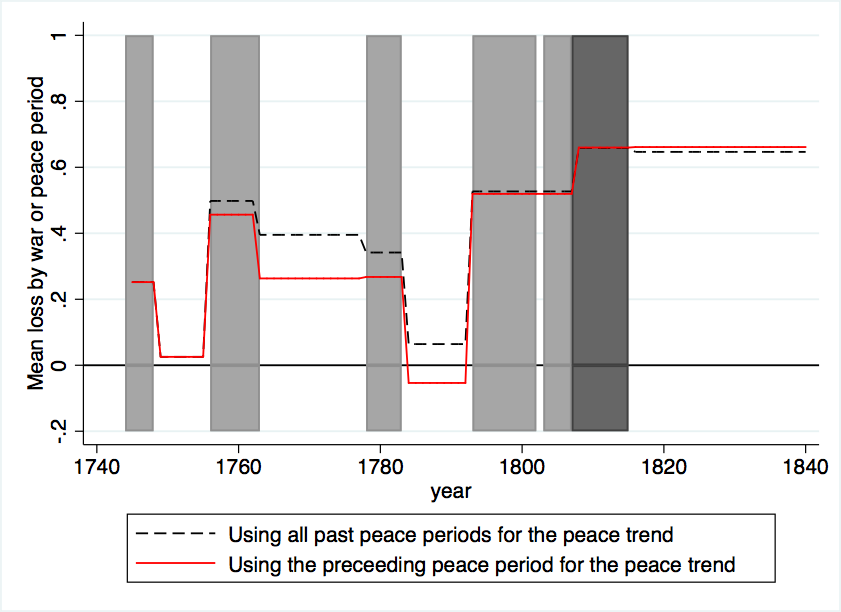
\includegraphics[scale=.3]{Mean_loss_function.png}
\end{figure}
\end{center}
These two figures reveal that the peace percentage loss of the Seven Years Wars and that of the Napoleonic Wars, were comparable to wartime loss, as opposed to faster recoveries in other post-war periods.
What made these wars so effective in terms of trade disruption?
How are they different from other similar wars in the same century? \\
This is an important question important to understand the effect of wars in general, the geopolitical history of the eighteenth and nineteenth century and the globalization/deglobalization cycle from the 1490s to the 1840s. \\
%The existing literature on this topic comes to mixed results. \cite{barbieri1999sleeping} for example, analyse the impact of war from 1870 to 1992, and find that the general impact of conflict on trade is not particularly strong and mostly only temporary. \cite{anderton2001impact}, on the other hand, look at the effect of wars on global trade, and find that when major world power are at war significant pre and post war effects are observed. Finally, \cite{rahman2010fighting}, using British trade data from eighteenth century, finds that it is warfare between naval powers that brings disruption to trade. In contrast, the resilience of French trade has long been remarked by historians (\cite{riley_seven_1986}). \\
To answer this question we explore several different hypothesis. \\
The first possible explanation is naval supremacy.
British naval supremacy over France meant that Britain could blockade French ports and capture French ships in a more efficient way.
To verify this, we use the number of warships available to France, France and its allies, Great Britain, Great Britain and its allies and neutral as provided in \cite{modelski1988seapower}, as a proxy for naval supremacy.
What we find, however, is that the most favourable war for France and its allies, in terms of naval supremacy, was the Seven Years War.
This suggests that naval supremacy is not a sufficient explanation. \\ 
A second hypothesis is colony loss. We construct a measure to account for this.
This measure equals 1 when France had all its colonies, and gets reduced by an amount proportional to the value of forgone trade whenever a colony is lost.
As in the previous case, there seem to be a correlation with with the period of the Revolutionary \& Napoleonic Wars, but this does not contribute to explain the loss in trade during the Seven Years War. \\
Finally, we explore the hypothesis of the role of neutral trade during conflicts. 
While trying to destroy foe's shipping, the way the Neutrals were treated was important as the merchants from belligerent countries used a number of devices to "hide" their cargo as neutral cargo, and continue trade (see \citep{carriere1973negociants}, \cite{schnakenbourg2013guerre}). 
During the century, belligerent countries - especially Great Britain - tried to close off these ways for French trade to continue thanks to neutral shipping.
In 1756, during Seven Years War, the British tried to reduce French trade on neutral ships by introducing the \textit{Doctrine of Continuous Voyage} along with the \textit{Rule of War of 1756}, that stated that the very beginning of the journey and the very end should be taken into account to determine the nationality of the cargo.
They also claimed and exercised the right to seize neutral shipping to look for contraband.
The situation for neutral trade was not very different during the Revolutionnary \& Napoleonic wars, as France become more and more hostile to neutral shipping as a way to try and isolate Great Britain.\\
There seems to be a correspondence between the loss function and the degree to which neutral trade was curtailed. This suggests  that trade with neutrals is important in explaining the contrasting resilience of French trade after each of its war with Great-Britain.
We conclude that, even if it is reasonable to believe that all these factors were contributing to the loss in trade during conflicts, the critical point was strictly related to policy towards neutral countries.
British could efficiently curtail French trade only by blockading neutral countries.





\textbf{Keywords}: international trade, 18th century, France, neutral trade, warfare

\pagebreak

\renewcommand{\baselinestretch}{1.0}\normalsize
\bibliographystyle{apa}
\bibliography{How_to_wage_a_trade_war}

\end{document}